Lidský mozek je schopen se neustále přizpůsobovat měnícím se okolnostem a
požadavkům prostředí. Astronauti se musí aklimatizovat na zcela nové prostředí
podobně jako malé děti procházejí svými vývojovými fázemi. V podmínkách stavu
beztíže nebo mikrogravitace dochází mimo jiné k ovlivnění mozkových procesů.
Cílem kognitivních neurověd ve vesmíru je pochopit, jak mozek a mysl reagují na
tyto jedinečné okolní podmínky. První výzkumy v oblasti neurověd ve vesmíru byly
provedeny v roce 1962 během ruské mise Vostok-3. Na Zemi je oproti vesmíru možné
díky neurozobrazovacím technikám snadno studovat mozkovou aktivitu a kognitivní
funkce. Pro neurovědce i psychology je velmi důležité pochopit základní
neurokognitivní a neuropsychologické aspekty kosmického letu. Neefektivní
mentální výkon jedince či posádky je známou hrozbou pro vesmírné mise. Pozemský
výzkum zdůrazňuje nutnost porozumět kognitivním procesům, jelikož \gls{CL}
zhoršuje kognitivní a percepční motorické schopnosti. Srovnatelné dopady lze
předpokládat i při vesmírných misích v náročných \gls{ICE} podmínkách a
simulacích (analogové mise)~\cite{Torre2014}. Pro potřeby diplomové práce je
rozsáhlá kapitola kognitivních neurověd vymezena popisu kognitivní zátěže.

\subsection{Terminologie}
\label{subsection:terminologie_CL}
Obor kognitivních neurověd se nachází na pomezí psychologie a neurověd, ale
překrývá se s dalšími obory jako kognitivní a biologická psychologie, fyziologie
nebo neuropsychologie. Tyto obory často studují podobné procesy ale z jiného
pohledu a pomocí jiné metodiky. Synonymem oblasti kognitivních neurověd byl v
této práci zvolen termín neuropsychofyziologie pro usnadnění popisu
fyziologických změn v důsledku kognitivních procesů. Cílem této práce není
rozlišovat mezi jednotlivými obory ale zaměřit se na vědecké otázky z jejich
průniků, které jsou spojené s vlivem \gls{ICE} prostředí na člověka.

\subsection{Kognitivní zátěž}
\label{subsection:kognitivni_zatez}
Prvotní pojetí kognitivní zátěže (\gls{CL}, Cognitive Load) pochází z oblasti
výuky a vzdělávání, kterou se intenzivně zabýval Sweller et
al.~\cite{Sweller1988,Sweller1998,Sweller2010} kolem přelomu 19. a 20. století.
Sweller~\cite{Sweller1988} jako první formuloval teorii kognitivní zátěže
(\gls{CLT}, Cognitive Load Theory), podle které je \gls{CL} definována jako
zvýšené požadavky na ukládání a zpracování informací v pracovní paměti člověka.
Chen et al.~\cite{Chen2016} definoval kognitivní zátěž jako proměnnou, jež
určuje míru požadavků kladených úkolem na dostupné mentální zdroje pro
zpracování informací. Míra požadavků vychází z vnímané námahy při učení, myšlení
a uvažování jakožto ukazatel zatížení pracovní paměti během plnění úkolu. Tato
míra zároveň popisuje interakce mezi nároky na zpracování úkolu a lidskou
mentální výkonností~\cite{Haapalainen2010}. Ačkoli se definice kognitivní zátěže
v jednotlivých oborech mohou lišit, všechny mají jeden základní prvek: procento
využité kapacity lidské pracovní paměti. Na rozdíl od naší smyslové a dlouhodobé
paměti, které mohou v podstatě neomezeně zpracovávat informace, je tato kapacita
omezená~\cite{Vanneste2021}.

Chen et al.~\cite{Chen2016} publikoval, že vysoká kognitivní zátěž (kognitivní
přetížení) může mít negativní dopad na výkonnost pracovní paměti. Vliv
kognitivní zátěže zároveň ovlivňuje mozkové procesy a kognitivní přetížení
pravděpodobně bezprostředně předchází vyhoření~\cite{Vanneste2021}. Většina
kognitivních funkcí, jako je například selektivní pozornost nebo sebekontrola,
závisí na pracovní paměti. Pracovní paměť zahrnuje aktivní krátkodobé ukládání,
zpracování a manipulaci s informacemi a její efektivní fungování je kriticky
závislé na inhibičních nervových procesech. Nervové středisko pracovní paměti
sestává hlavně z distribuované sítě struktur zahrnující prefrontální kortex jako
důležité ohnisko. Variabilita srdeční frekvence (\gls{HRV}) souvisí s aktivitou
prefrontální kůry a je inverzně spojena s aktivitou subkortikálních struktur
jako je amygdala~\cite{Thayer2009}. Vliv kognitivní zátěže se také promítá do
elektrodermální (\gls{EDA}) a respirační (\gls{RSP})
aktivity~\cite{Mogilever2018}. Díky periferním biologickým signálům se tedy
naskytuje jednoduší možnost hodnocení či predikce kognitivních procesů bez
nutnosti použití realizačně a finančně náročnějších neurozobrazovacích metod
nebo elektroencefalografie (\gls{EEG}). Detailněji jsou fyziologické změny
spojené s vlivem \gls{CL} popsány v následující sekci.

\subsection{Fyziologické projevy}
\label{subsec:fyziologicke_projevy_CL}
Z předchozího textu již může být zřejmé, že kognitivní zátěž je velmi úzce
spojená s fyziologickými změnami v lidském organismu. U jedince, kde dojde k
stimulaci CL, může docházet k řadě změn, například v mozkové aktivitě, krevním
tlaku, srdečním rytmu, rychlosti pulzní vlny, dýchaní nebo činnosti potních
žláz~\cite{Vanneste2021,Haapalainen2010,Thayer2009,Gjoreski2017,Cruz2019,Brouwer2015}.
Vybrané fyziologické funkce, do kterých se po promítá kognitivní zátěž, jsou
společně s jejich krátkým popisem a neurobiologickým vztahem uvedeny v
Tabulce~\ref{tab:prehled_fyziologicke_projevy_CL_tab1}. Tabulka zároveň
poukazuje na rozdílné vztahy fyziologických parametrů s kognitivní zátěží.

\begin{table}[ht]
    % \setlength{\tabcolsep}{10pt}
    \renewcommand{\arraystretch}{1.5}
    \centering
    \begin{threeparttable}
        \caption{Přehled vybraných nejčastěji studovaných fyziologických změn
            a stručné teoretické zdůvodnění jejich souvislosti s kognitivní zátěží
            (Upraveno a převzato z~\cite{Vanneste2021})}
        \label{tab:prehled_fyziologicke_projevy_CL_tab1}
        \scriptsize
        \begin{tabular}{p{3cm}p{11cm}}
            \toprule
            Fyziologická funkce & Stručný popis a teoretické zdůvodnění předpokládaného vztahu mezi fyziologickým měřením a kognitivní zátěží
            \\ \midrule
            EEG                 & \textit{Popis}: \gls{EEG} umožňuje měřit mozkovou aktivitu neinvazivně. Provedení spektrální analýzy naměřených rozdílů elektrických potenciálů umožňuje analyzovat výkon různých frekvenčních pásem, která jsou v signálu\newline
            \rule{0pt}{2.5ex}\noindent
            \textit{Hypotéza}: Zvýšení kognitivní zátěže lze měřit zvýšením mozkové aktivity, tj. oscilací v určitém frekvenčním pásmu s větší amplitudou~\cite{Antonenko2010}
            \\
            Eye-tracking        & \textit{Popis}: Měření průměru zornice, latence mrknutí a charakteristik sakád\newline
            \rule{0pt}{2.5ex}\noindent
            \textit{Hypotéza}: Sledování očí bylo v předchozích studiích spojeno s kognitivní zátěží prostřednictvím neurobiologických mechanismů, jako je inervace neuronů autonomního nervového systému radiálními vlákny duhovky~\cite{Wel2018}
            \\
            EDA                 & \textit{Popis}: Elektrodermální aktivita, hodnotí elektrické charakteristiky kůže, aby bylo možné odvodit změny vlivem sympatického nervového systému.\newline
            \rule{0pt}{2.5ex}\noindent
            \textit{Hypotéza}: Kognitivní zátěž má vliv na stres nebo vzrušení a vede ke zvýšení kožní vodivosti~\cite{Setz2010}
            \\
            Teplota pokožky     & \textit{Popis}: Měření teploty vnějšího povrchu lidského těla\newline
            \rule{0pt}{2.5ex}\noindent
            \textit{Hypotéza}: Kognitivní zátěž má vliv na stres nebo vzrušení a vede k vazokonstrikci, což snižuje teplotu kůže~\cite{Herborn2015}
            \\
            EKG                 & \textit{Popis}: Srdeční frekvenci a variabilitu srdeční frekvence lze hodnotit pomocí elektrokardiogramu nebo fotopletysmografie\newline
            \rule{0pt}{2.5ex}\noindent
            \textit{Hypotéza}: Tepová frekvence je měřítkem aktivity sympatického i parasympatického autonomního nervového systému. Stres nebo vzrušení způsobí zvýšení krevního tlaku a snížení variability srdeční frekvence~\cite{Jercic2020,Solhjoo2019}
            \\
            RSP                 & \textit{Popis}: Kognitivní zátěž vede ke zrychlenému dýchání a vyšší minutové ventilaci, přičemž dechová amplituda zůstává stejná\newline
            \rule{0pt}{2.5ex}\noindent
            \textit{Hypotéza}: Při soustředění pozornosti nebo plnění náročného úkolu dochází ke změnám v dýchání~\cite{Grassmann2016}
            \\
            \bottomrule
        \end{tabular}
    \end{threeparttable}
\end{table}

Příkladem rozdílností může být EEG, u kterého je vztah s kognitivní zátěží
přímější než u srdeční nebo elektrodermální aktivity. Hodnocení pomocí tohoto
biosignálu je tedy v některých případech spolehlivější. Pouze v některých,
protože se vychází z předpokladu, že veškeré změny v kognitivních funkcích
člověka se odrážejí v jeho fyziologii~\cite{Vanneste2021}. To znamená, že žádná
měřicí technika nemůže sama o sobě zachytit všechny aspekty kognitivních funkcí
nebo o nich jednoznačně vypovídat. Problematika těchto vztahů je nadále
rozebírána v kapitole~\ref{sec:neurovisceralni_integrace}. Na tuto vícerozměrnou
povahu kognitivní zátěže poukázal Kramer et al.~\cite{Kramer1991}. Dále
definoval kritéria: citlivost, diagnostičnost, rušivost, spolehlivost a obecnost
použití, v rámci kterých bude mít každé fyziologické měření jinou povahu. V
případě kognitivní zátěže a její spolehlivém hodnocení z fyziologických projevů
je proto vhodný multimodální\footnote{Multimodálním přístupem je myšleno využití
více biosignálů.} přístup, který může poskytnout její robustnější
reprezentaci~\cite{Chen2016}.

\subsection{Detekce kognitivní zátěže}
\label{subsec:detekce_CL}
Detekce kognitivní zátěže pomocí periferních biosignálů patří mezi tři
nejčastěji používané způsoby včetně subjektivního hodnocení a hodnocení založené
na výkonnosti jedince. Subjektivní hodnocení vychází z předpokladu, že hodnocený
subjekt je schopen vnímat své vlastní kognitivní procesy a informovat o případně
kognitivní zátěží nebo o množství vynaloženého mentálního
úsilí~\cite{Wang2019,Schnotz2007}. K subjektivnímu hodnocení se dále využívají
specifické dotazníky, mezi které patří například NASA-TLX. Jedná se o
vícerozměrnou stupnici používanou k měření pracovní zátěže operátorů v rámci
úkonů, například během vesmírných analogových misí~\cite{Sandra2006}. Tyto
metody ale nejsou předmětem této práce a již byly detailně popsány
v~\cite{Schnotz2007}.

\begin{figure}[!htb]
    \begin{center}
        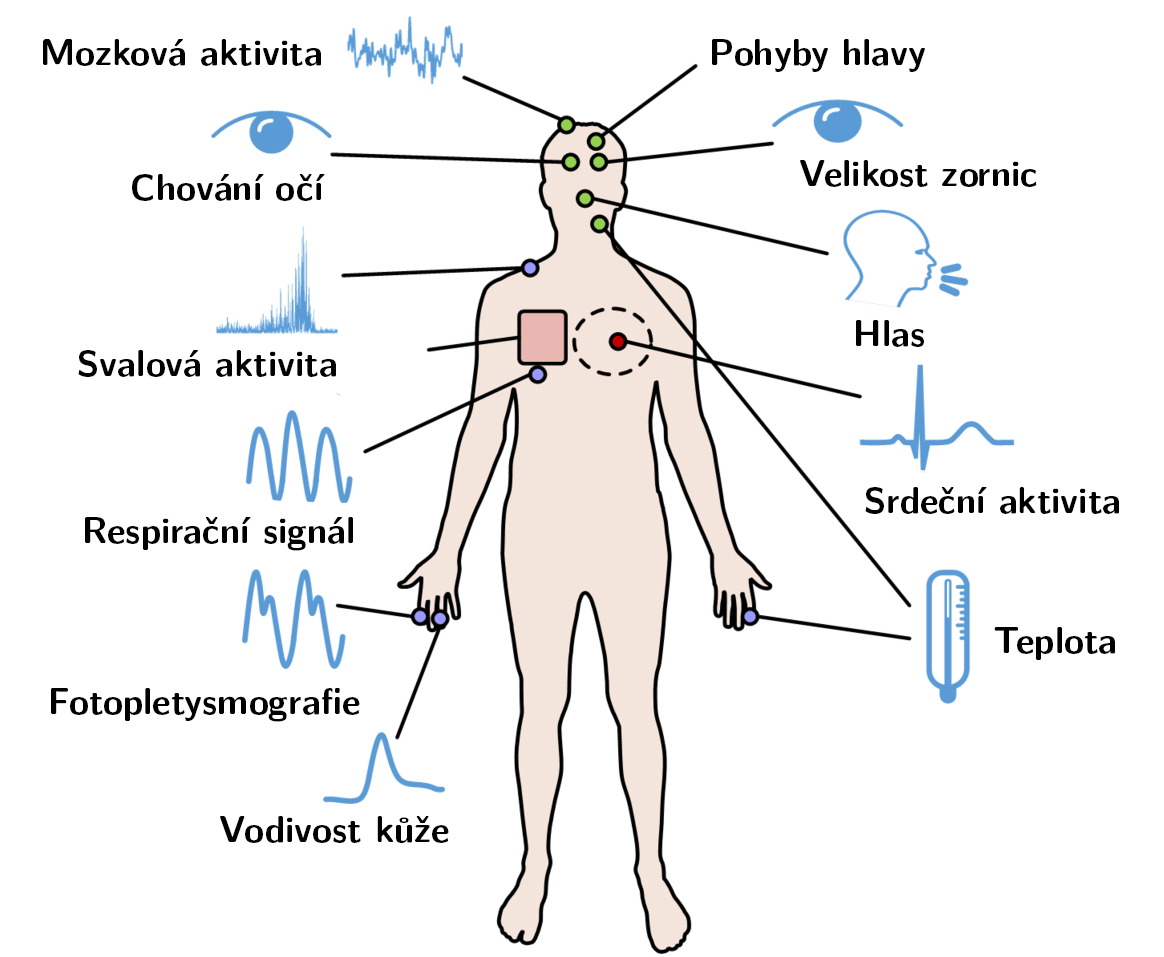
\includegraphics[width=0.85\linewidth]{figures/physiological_measures}
        \caption{Vybrané proměnné související s \gls{CL} (Přeloženo a převzato
            z~\cite{Giannakakis2022})}
        \label{fig:physiological_measures}
    \end{center}
\end{figure}

Na kognitivní zátěž lze nahlížet jako na multidimenzionální konstrukt, který
reprezentuje zátěž vyvinutou na jedince~\cite{Wang2019}. Zároveň se efekt
stimulace kognitivních funkcí u každého jedince projevuje jinak. Nelze tedy
vytvořit žádnou univerzální metodu, která by byla schopná stejně spolehlivě
detekovat kognitivní zátěž u různých subjektů. Proto se v tomto odvětví nabízejí
a velmi často využívají metody strojového učení v rámci kterých nachází výhodné
uplatnění dříve zmíněný multimodální přístup. Biologická data využívaná pro
účely detekce \gls{CL} lze vidět na Obr.~\ref{fig:physiological_measures}.

Vzhledem k tomu, že je strojové učení širokou oblastí, byla tomuto tématu
věnována samostatná sekce~\ref{sec:machine_learning}. Od roku 2010 je hojně
využívána metoda učení s učitelem (viz~\ref{subsubsec:supervised_learning}) pro
účely klasifikace různých patologických stavů a symptomů~\cite{Ishaque2021}.
Nejčastěji využívaným biosignálem je srdeční aktivita, konkrétně variabilita
srdeční frekvence, které se často používá v kombinaci s elektrodermální
aktivitou~\cite{Wang2019}. Použité příznaky pro klasifikaci (anglicky features)
však hrají důležitou roli při rozlišování základní funkce spojené s jakýmkoli
fyziologickým signálem. Z variability srdeční frekvence je v současnosti možné
vypočítat desítky parametrů, resp. příznaků, se kterými je v těchto úlohách
nutné velmi opatrně zacházet. Jednotlivé \gls{HRV} parametry společně s jejich
pravděpodobným významem byly již popsány
v~\cite{Haapalainen2010,Rohila2020,Pham2021,Bouny2021}. Blíže je problematika
\gls{HRV} parametrů popsána v samotné podkapitole~\ref{subsec:hrv_indices}.

Dříve mezi často používané metody pro účely klasifikace patřili hlavně
rozhodovací stromy (\gls{DT}), lineární diskriminační analýza (\gls{LDA}) nebo
metoda podpůrných vektorů (\gls{SVM})~\cite{Ishaque2021}. Od roku 2018 se ve
výzkumu HRV však stále častěji používá hluboké učení, jehož cílem je zlepšit
automatickou klasifikaci v reálném čase. Tyto techniky poskytují efektivnější
způsob extrakce relevantních informací a zvyšují přesnost klasifikace a současně
snižují počet příznaků potřebných pro klasifikaci v reálném
čase~\cite{Hwang2018,He2019}. O rok později se stalo novým trendem používání
technik učení bez učitele pro klasifikaci psychického stresu s využitím
technologie autoenkodéru~\cite{Oskooei2019}. Dále se mimo jiné začaly hojně
používat samoorganizující mapy (\gls{SOM}), které dokáží efektivně redukovat
dimenzionalitu dat a zároveň indikovat nejcennější\footnote{Implikuje jak moc
přispívá každý příznak k predikci modelu.} příznaky pro klasifikaci kognitivní
zátěže s vysokou přesností~\cite{Cho2017}. Jelikož ale neexistuje žádný
konsensus jak předzpracovávat biosignály, jaké využít příznaky nebo z jaké
metodiky pro detekci CL vycházet, tak se stále zkouší nejasné variace různých
algoritmů se snahou zvýšit skóre predikce. Velkým problémem je také nedostatek
veřejně dostupných dat pro tyto účely.

% \begin{table}[h]
%     \centering
%     \caption{Veřejně dostupné datasety sledující kognitivní zátěž (Upraveno a
%         převzato z~\cite{Gjoreski2020})}
%     \label{tab:cl_datasets}
%     \scriptsize
%     \begin{tabular}{lcp{9cm}}
%         \toprule
%         \textbf{Dataset}      & \textbf{Probandi} & \textbf{Biosignály}                                                          \\ \midrule
%         Ascertain             & 58                & ECG, EDA, EEG, aktivační jednotky obličeje                                   \\
%         Amigos                & 40                & EEG, ECG, GSR, video obličeje                                                \\
%         DEAP                  & 32                & ECG, EDA, EEG, EMG, EOG, RSP, TEMP, video obličeje                           \\
%         DECAF-hudba           & 30                & ECG, EMG, EOG, MEG, near-infrared video obličeje                             \\
%         DECAF-video           & 30                & ECG, EMG, EOG, MEG, near-infrared video obličeje                             \\
%         Mahnob                & 30                & ECG, EDA EEG, RSP, TEMP, video, sledování očí, zvuk                          \\
%         Emotions              & 1                 & ECG, EDA, EMG, RSP                                                           \\
%         Laughter              & 34                & ACC, EDA, PPG, TEMP                                                          \\ \midrule
%         Pracovní zátěž řidiče & 10                & GSR, HR, TEMP                                                                \\
%         Řidičský stres        & 24                & ECG, EDA, EMG, RESP                                                          \\
%         Rozptýlení řidiče     & 64                & GSR, HR, TEMP ECG, EDA, EMG, RSP EDA,HR, RSP, výrazy obličeje, sledování očí \\ \midrule
%         \textbf{CLAS}         & 59                & ACC, ECG, PPG, EDA                                                           \\
%         Stress-math           & 21                & ACC, EDA, HR, TEMP, BVP ACC, EDA, HR, TEMP, BVP                              \\
%         Non-EEG               & 20                & ACC, EDA, HR, TEMP, BVP ACC, EDA, HR, TEMP, SpO2                             \\
%         \textbf{WESAD}        & 15                & ACC, EDA, TEMP, BVP, EMG, RSP                                                \\ \midrule
%         CogLoad               & 23                & ACC, EDA, TEMP, RR                                                           \\
%         Snake                 & 23                & ACC, EDA, TEMP, RR                                                           \\ \bottomrule
%     \end{tabular}
% \end{table}